\usepackage[utf8]{inputenc}
\bibliographystyle{apalike}
\usepackage{bibentry}
\nobibliography*
\usepackage{slovak}
\usepackage{tikz}
\usetikzlibrary{arrows,positioning}
\usetheme{Warsaw}
\title{Biologicky motivované \\výpočtové modely}
\author[Mgr. Michal Kováč]{Mgr. Michal Kováč\\{\small Školiteľ: doc. RNDr. Damas Gruska, PhD.}}
\institute{FMFI UK}
\date{17.1.2018}
\begin{document}
% \renewcommand{\pause}{}

\begin{frame}[t]
\titlepage
\end{frame}

\begin{frame}
\tableofcontents
\end{frame}
\note{
  V úvode prezentácie vám predstavím rôzne výpočtové modely motivované biologiou. Najviac sme sa venovali P systémom, preto budem pokračovať formálnou definíciou a prehľadom rôznych variantov P systémov.

  V druhej časti predstavím 4 témy nášho výskumu, z čoho 3 články boli publikované. V našej práci sme skúmali viaceré varianty P systémov a to konkrétne Sekvenčné P systémy s inhibítormi, Sekvenčné P systémy s aktívnymi membránami, Sekvenčné P systémy s množinami namiesto multimnožín, z čoho všetky spomenuté témy boli publikované. Dalším variantom P systémov, ktorým sme sa zaoberali bola Detekcia prázdnosti membrán.
}

\section{Prehľad problematiky} % (fold)
\label{sec:prehlad_problematiky}

\subsection{Prehľad modelov} % (fold)
\label{sub:prehlad_modelov}

\begin{frame}[t]\frametitle{Biologicky motivované \\výpočtové modely}
  Dvojaké uplatnenie:
  \begin{itemize}
    \item reálne modely živých systémov
    \begin{itemize}
      \item virtuálne biologické experimenty
      \item verifikácia správnosti chápania ich činností
    \end{itemize}
    \item modely na popis iných systémov
  \end{itemize}
\end{frame}
\note{
  Biologicky motivované výpočtové modely majú dvojaké uplatnenie.

  Jednak v rámci biológie môžu slúžiť ako reálne modely správania sa živých systémov, na ktorých môžeme robiť rôzne virtuálne biologické experimenty, prípadne verifikovať správnosť nášho chápania ich biologickej činnosti.

  Na druhej strane môžu slúžiť ako modely na popis aj iných ako biologických systémov, čo otvára rad teoretických informatických otázok, napr. výpočtová sila alebo analýza behaviorálnych vlastností.
}

\begin{frame}[t]\frametitle{Biologicky motivované \\výpočtové modely}
  \begin{itemize}
    \item Neurónové siete (od 1943)
    \item Celulárne automaty (od 1968)
    \item Evolučné algoritmy (od 1954)
    \item L systémy (od 1968)
    \item Swarm Intelligence (od 1989)
    \item P systémy (od 1998) \cite{Paun98}
    \item \dots
  \end{itemize}
\end{frame}
\note{
  Dlho skúmané modely ako neurónové siete, celulárne automaty, evolučné algoritmy, L systémy, či swarm intelligence, si už našli svoje uplatnenie v praxi, kým membránové systémy sú ešte len v začiatkoch svojho vývoja.
}

% subsection prehlad_modelov (end)

\subsection{P systémy} % (fold)
\label{sub:p_systemy}

\begin{frame}[t]\frametitle{Membránová štruktúra}
  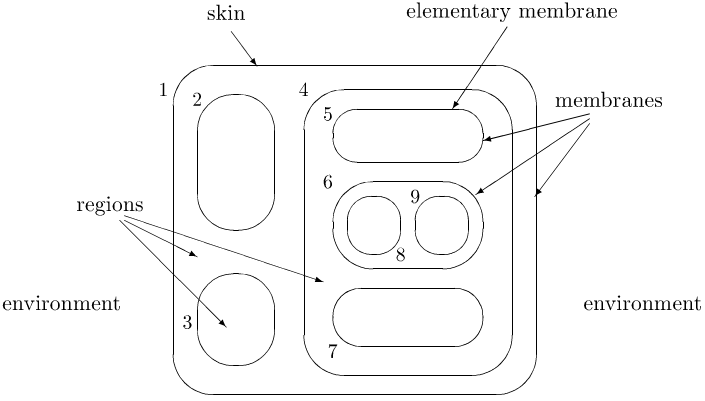
\includegraphics[width=0.7\textwidth]{membrane_structure.png}
  \hfill
  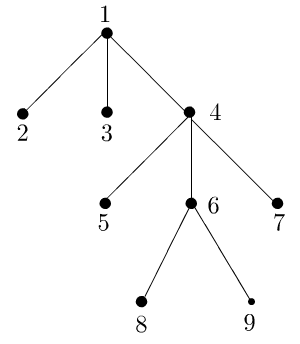
\includegraphics[width=0.3\textwidth]{membrane_tree.png}
  \pause
  \begin{itemize}
    \item Multimnožiny
    \pause
    \item Pravidlá
  \end{itemize}

\end{frame}
\note{
  Membránové systémy sú inšpirované bunkami. Základom je preto membránová štruktúra, ktorá pozostáva z regiónov, ktoré sú oddelené membránami. Tvorí to hierarchickú štruktúru, ktorá sa dá zobraziť aj ako strom.

  NEXT SLIDE

  Obsahom regionov je multimnožina objektov, ktoré v realite predstavujú napr. molekuly, vírusy, enzýmy alebo proteíny.

  NEXT SLIDE

  Objekty medzi sebou môžu interagovať. Táto interakcia je definovaná prepisovacími pravidlami.
}

\begin{frame}[t]\frametitle{Prepisovacie pravidlá}
  $u\rightarrow v$, where
  \begin{itemize}
    \item $u\in\mathbb{N}^\Sigma$
    \pause
    \item $v=v^\prime$ or $v=v^\prime\delta$, where $\delta\notin\Sigma$
    \item $v^\prime\in\mathbb{N}^{\Sigma\times(\{here, out\}\cup\{in_j|1\leq j\leq m\})}$
  \end{itemize}
\end{frame}
\note{
  Prepisovacie pravidlá majú ľavú a pravú stranu. Na ľavej strane sú reaktanty, čo je multimnožina objektov.

  NEXT SLIDE

  Na pravej strane sú produkty, čo je multimnožina objektov, pričom pre každý objekt sa definuje, či ostáva v aktuálnom regione, alebo ide cez membránu do vonkajšieho regionu alebo cez membránu s daný označením do vnútorného regionu.

  Delta je špeciálny symbol, ktorý nepatrí abecede, ktorý ked je prítomný, tak po aplikovaní pravidla sa rozpustí membrána, v ktorej sa pravidlo aplikovalo a obsah membrány sa vyleje von.

  Pravidlo je aplikovateľné v danom regione, ak sú reaktanty obsiahnuté v multimnožine objektov, ktorá sa aktuálne nachádza v danom regione.  
}

\begin{frame}[t]\frametitle{Varianty pravidiel}
  $u\rightarrow v$
  \begin{itemize}
    \item Kooperatívne ($u\in\mathbb{N}^\Sigma$) (PsRE \cite{Paun98})
    \pause
    \item Nekooperatívne ($u\in\Sigma$) (PsCF \cite{Sburlan05dragos})
    \pause
    \item Nekooperatívne s inhibítormi ($u \rightarrow v\ |_{\neg{Inh}}, Inh\subseteq\Sigma$) (PsET0L \cite{Ionescu:jucs_10_5:on_p_systems_with})
    \pause
    \item Katalytické ($cu \rightarrow cv, u\in\Sigma, c\in C\subseteq\Sigma$)
    \begin{itemize}
      \item s 2 katalyzátormi (PsRE \cite{Freund2005TwoCatalysts})
      \item s 1 katalyzátorom (otvorený problém)
      \item s 1 katalyzátorom a inhibítormi (PsRE \cite{Ionescu:jucs_10_5:on_p_systems_with})
    \end{itemize}
  \end{itemize}
\end{frame}
\note{
  Literatúra spomína rôzne spôsoby definovania prepisovacieho pravidla. Pôvodná definícia, ktorú uvádza Paun, používa kooperatívne pravidlá v znení, ako som uviedol. Takto definované P systémy sú Turingovsky úplné.

  NEXT SLIDE

  Nekooperatívne pravidlá neumožňujú interakciu medzi objektami, takže na ľavej strane je vždy iba jeden objekt. Takto definované P systémy sú ekvivalentné Parikhovmu zobrazeniu bezkontextových jazykov.

  NEXT SLIDE

  Pravidlá s inhibítormi umožňujú špecifikovať množinu objektov, inhibítorov, z ktorých ak aspoň jeden je prítomný v regione, tak dané pravidlo sa nemôže uplatniť. Takto definované P systémy sú ekvivalentné Parikhovmu zobrazeniu triedy jazykov ET0L.
}
\newpage
\note{
  Katalytické pravidlá umožňujú objektom interagovať iba s objektom z množiny katalizátorov.
  Dva katalyzátory stačia na Turingovskú úplnosť. Výpočtovú silu P systémov s jedným katalyzátorom nevieme zaradiť, je to otvorený problém. Ak ale umožníme pravidlá s inhibítormi, dosiahneme Turingovskú úplnosť.
}
    
\begin{frame}[t]\frametitle{Výpočet a jazyk}
  \begin{itemize}
    \item Krok výpočtu
    \begin{itemize}
      \item Sekvenčný
      \item Paralelný
      \item Maximálne paralelný
    \end{itemize}
    \pause
    \item Jazyk
    \begin{itemize}
      \item Generatívny mód: postupnosť objektov vypustených do okolitého prostredia
      \pause
      \item Akceptačný mód: daná konfigurácia je akceptovaná, ak sa systém vie dostať do stavu, kde sa už nedá použiť žiadne pravidlo
    \end{itemize}
  \end{itemize}
\end{frame}
\note{
  Postupné uplatňovanie pravidiel definuje výpočet.

  V jednom kroku výpočtu sa uplatní:
  \begin{itemize}
    \itemsep0em
    \item presne jedno pravidlo (sekv. mod)
    \item aspoň jedno pravidlo (paralelný mod)
    \item maximálna multimnožina pravidiel
  \end{itemize}

  V pôvodnej definícii, ktorú uvádza Paun, sa používa maximálny paralelizmus.
}
\newpage
\note{
  P systém definuje jazyk rôznymi spôsobmi. Môže to byť jazyk nad slovami - postupnosťami objektov alebo jazyk nad multimnožinami.
  
  V generatívnom mode môžeme zobrať objekty vypustené do prostredia počas výpočtu a túto postupnosť objektov alebo multimnožinu objektov zahrnúť do jazyka.
  Kedže pre daný P systém vdaka nedeterminizmu existuje viac možných výpočtov, veľkosť definovaného jazyka môže byť aj väčsia ako 1.
}
\newpage
\note{
  V akceptačnom mode môžeme pre nejaké zobrazenie slov alebo multimnožín na konfigurácie P systému pre dané slovo spustiť výpočet s konfiguráciou, ktorá je obrazom toho slova podľa daného zobrazenia.
  
  V akceptačnom mode môžeme pre nejaké zobrazenie $f$ slov na konfigurácie P systému pre dané slovo $w$ spustiť výpočet s konfiguráciou $f(w)$.

  Ak tento výpočet zastaví, teda sa už nedá použiť žiadne dalšie pravidlo, dané slovo alebo multimnožinu zahrnieme do jazyka.
}

\begin{frame}[t]\frametitle{Sekvenčné P systémy}
  \begin{itemize}
    \item Maximálny paralelizmus vs. sekvenčný mód
    \pause
    \item Sekvenčné P systémy s kooperatívnymi pravidlami (VASS \cite{Dang:2005:Sequential})
    \pause
    \begin{itemize}
      \item s prioritami (RE \cite{Dang:2005:Sequential})
      \pause
      \item s aktívnymi membránami (RE \cite{Dang:2005:Sequential})
      \pause
      \item {\bf s inhibítormi (RE \cite{Kovac14})}
    \end{itemize}
    \pause
    
  \end{itemize}
\end{frame}
\note{}

% subsection p_systemy (end)

% section prehlad_problematiky (end)

\section{Skúmané varianty P systémov} % (fold)
\label{sec:sk_man_varianty_p_syst_mov}

\subsection{Sekvenčné P systémy s inhibítormi} % (fold)
\label{sub:sekven_n_p_syst_my_s_inhib_tormi}

\begin{frame}[t]\frametitle{Sekvenčné P systémy s inhibítormi}
  \begin{itemize}
    \item \bibentry{Kovac14}
  \end{itemize}
\end{frame}


\begin{frame}[t]\frametitle{Prehľad simulácie pre akceptačný mód}
  \begin{itemize}
    \item Simulácia registrového stroja
    \pause
    \item Obsah registra $x$ sa reprezentuje početnosťou objektu $x$
    \item Objekt pre každú inštrukciu
    \pause
    \item SUB inštrukcia sa simuluje pomocou inhibítora
    \begin{itemize}
      \item $i: SUB(x,j,k)$
      \item $ix\rightarrow j$
      \item $i\rightarrow k|_{\neg{x}}$
    \end{itemize}
  \end{itemize}
\end{frame}
\note{}

\begin{frame}[t]\frametitle{Prehľad simulácie pre generatívny mód}
  \begin{itemize}
    \item Simulácia maximálne paralelného P systému $\Pi_1$ pomocou sekvenčného P systému s inhibítormi $\Pi_2$.
    \pause
    \item Každý maximálne paralelný krok $\Pi_1$ simulujeme sekvenčnými krokmi $\Pi_2$.
    \pause
    \item Produkty si označujeme, aby neboli použité, kým neskončí daný maximálne paralelný krok.
    \pause
    \item Pomocou inhibítorov zistíme moment, kedy sa už v $\Pi_2$ nedá aplikovať žiadne pravidlo, aby sa mohol simulovať ďalší maximálne paralelný krok.
  \end{itemize}
\end{frame}
\note{}

% subsection sekven_n_p_syst_my_s_inhib_tormi (end)

\subsection{Sekvenčné P systémy s aktívnymi membránami} % (fold)
\label{sub:sekven_n_p_syst_my_s_akt_vnymi_membr_nami}

\begin{frame}[t]\frametitle{Sekvenčné P systémy s aktívnymi membránami}
  \begin{itemize}
    \item Bez limitu počtu aplikovaní pravidla na vytvorenie membrány (RE \cite{Ibarra05Active})
    \pause
    \item \bibentry{Kovac15Active}
  \end{itemize}

  
\end{frame}

\begin{frame}[t]\frametitle{Problém zastavenia}
  \begin{itemize}
    \item Problém zastavenia je definovaný pre deterministické modely
    \pause
    \item Zovšeobecnenie: Existencia (ne)konečného výpočtu
  \end{itemize}

\end{frame}
\note{}

\begin{frame}[t]\frametitle{Existencia nekonečného výpočtu}
  \begin{itemize}
    \item Graf dosiahnuteľnosti
    \pause
    \item Čiastočné usporiadanie $\leq$:
    \begin{itemize}
      \item $C_1 \leq C_2 \Rightarrow$ každé pravidlo v $C_1$ je aplikovateľné v $C_2$.
      \pause
      \item Pre každú nekonečnú postupnosť konfigurácií existuje $C_1, C_2$: $C_1 \rightarrow^* C_2$ a $C_1 \leq C_2$.
    \end{itemize}
    \pause
    \item Dicksonova lemma: Pre každú nekonečnú postupnosť n-tíc nad $\mathbb{N}$ $\{a_i\}_{i=0}^\infty$ existujú $i<j$: $a_i\leq a_j$
  \end{itemize}
\end{frame}

\begin{frame}[t]{Algoritmus rozhodujúci existenciu nekonečného výpočtu}
  \begin{itemize}
    \item Traverzuj graf dosiahnuteľnosti
    \item Dosiahnutá konfigurácia $C_2$, taká, že na ceste z počiatočnej konfigurácie existuje $C_1\leq C_2\Rightarrow$ YES.
    \item Ak traverzovanie skončilo $\Rightarrow$ NO.
  \end{itemize}
\end{frame}

\begin{frame}[t]{Existencia konečného výpočtu}
  \begin{itemize}
    \item Pre daný P systém $\Pi$ a danú konfiguráciu $C$ vieme zostrojiť P systém $\Pi^\prime: \exists$ konečný výpočet $\Pi^\prime\Leftrightarrow C$ je dosiahnuteľná v $\Pi$.  
  \end{itemize}  
\end{frame}

% subsection detekcia_pr_zdnosti_membr_n (end)

\subsection{Sekvenčné P systémy s množinami namiesto multimnožín} % (fold)
\label{sub:sekven_n_p_syst_my_s_mno_inami_namiesto_multimno_n}

\begin{frame}[t]{Sekvenčné P systémy s množinami namiesto multimnožín}
  \begin{itemize}
    \item \bibentry{Kovac15Set}
  \end{itemize}
\end{frame}

\begin{frame}[t]{Nevýhody používania multimnožín}
  \begin{itemize}
    \item Nakoľko realistické je reprezentovať presný počet objektov?
    \item Nepraktická analýza kvôli veľkosti stavového priestoru
  \end{itemize}
\end{frame}

\begin{frame}[t]\frametitle{P systémy s množinami objektov}
  \begin{itemize}
    \item Alhazov \cite{Alhazov05WithoutMultiplicities}: počty objektov sa ignorujú
    \pause
    \begin{itemize}
      \item Maximálny paralelizmus $\Rightarrow$ determinizmus.
      \pause
      \item Ekvivalencia s konečnostavovými automatmi.
      \pause
      \item S aktívnymi membránami je model univerzálny.
      \pause
    \end{itemize}
    \item Kleijn, Koutny \cite{Kleijn11SetMembrane}: ``min-enabled'' computational step (= sekvenčný mód)
    \pause
    \begin{itemize}
      \item Ekvivalencia s konečnostavovými automatmi.
    \end{itemize}
    \pause
    \item Vlastnosti:
    \begin{itemize}
      \item Pravidlá bez konfliktu (objekty sa môžu zúčastniť ako reaktanty súčasne vo viacerých pravidlách).
      \item Ak je objekt použitý aspoň v jednom pravidle ako reaktant, bude spotrebovaný.
    \end{itemize}
  \end{itemize}
\end{frame}
\note{}

\begin{frame}[t]\frametitle{Sekvenčné P systémy s množinami objektov a aktívnymi membránami}
  \begin{itemize}
    \item $\Pi = (\Sigma, C_0, R_1, \ldots R_m)$
    \pause
    \item $C = (T, l, c)$
    \begin{itemize}
      \item $l: V(T) \rightarrow \{1, \ldots, m\}$
      \item $c: V(T) \rightarrow 2^\Sigma$
    \end{itemize}
    \pause
    \item Pravidlá
    \begin{itemize}
      \item $u\rightarrow w$
      \item $u\rightarrow w\delta$
      \item $u\rightarrow [_j v_1]_j v_2$,

      kde $u \in \Sigma, |u|\geq 1$, $v_1,v_2\in \mathbb{N}$ a $w\in (\Sigma\times\{\cdot, \uparrow, \downarrow_{j}\})$
    \end{itemize}

  \end{itemize}
\end{frame}
\note{}

\begin{frame}[t]\frametitle{Iné spôsoby vytvárania membrány}
  \begin{itemize}
    \item Problémy pôvodnej definície:
    \begin{itemize}
      \item Vytváranie membrány, ktorá už existuje
      \item Posielanie objektu do neexistujúcej membrány
    \end{itemize}
    \pause
    \item Inject-or-create
    \pause
    \item Wrap-or-create
  \end{itemize}
\end{frame}

\begin{frame}[t]\frametitle{Simulácia registrového stroja}
  \begin{center}
    \begin{tabular}{c|c|c}
      \hline
      & membrány & čas \\ \hline
      original & $O(n)$ & $O(n)$ \\ \hline
      \pause
      original & $O(log(n))$ & $O(log(n))$ \\ \hline
      \pause
      inject-or-create & $O(log(n))$ & $O(log(n))$ \\ \hline
      \pause
      wrap-or-create & $O(n)$ & $O(1)$ \\ \hline
    \end{tabular}
  \end{center}
\end{frame}

% subsection sekven_n_p_syst_my_s_mno_inami_namiesto_multimno_n (end)

% subsection sekven_n_p_syst_my_s_akt_vnymi_membr_nami (end)

\subsection{Detekcia prázdnosti membrán} % (fold)
\label{sub:detekcia_pr_zdnosti_membr_n}

\begin{frame}[t]{Detekcia prázdnosti membrán}
  \begin{itemize}
    \item Objekty vyhýbajúce sa prázdnym membránam
    \pause
    \item Mutovanie objektov pri poslaní do prázdnej membrány
    \pause
    \item Objekt reprezetujúci vákuum
  \end{itemize}  
\end{frame}

% section sk_man_varianty_p_syst_mov (end)


\begin{frame}[plain]
\begin{center}
  Ďakujem za pozornosť
\end{center}
\end{frame}

\begin{frame}[t]{Vyjadrenia k posudkom}
  \begin{itemize}
    \item Štandardnou motiváciou pre skúmanie týchto modelov je potenciál vysokého paralelizmu. Práca je príliš zameraná na sekvenčný mód, ktorý úplne eliminuje potenciál tohto modelu.
    \pause
    \item V práci sa hovorí o slabých rozšíreniach sekvenčných P systémov s čiastočnými výsledkami. Aký je v uvedenom smere pokrok od podania dizertácie?
  \end{itemize}
\end{frame}

\newsavebox\mytempbib
\savebox\mytempbib{\parbox{\textwidth}{\bibliography{obhajoba}}}

\end{document}